\chapter{高维几何}

\section{在高维单位球中采样}

我们用 $V(d,r)$ 表示 $\mathbb{R}^{d}$ 中的半径为 $r$ 的球的体积，单位球的体积则简记作 $V(d)$。易见：
\[
	V(d,r) = r^{d} \cdot V(d)
\]
在接下来的部分中，我们会多次遇到“从单位球中随机取一个点”的说法，所以我们需要弄清怎样在 $d$ 维单位球中均匀地采样。先考虑如何在球的表面均匀采样：

\begin{algorithm}[h]
    \caption{单位球表面的采样}
    \begin{algorithmic}[1]
        \For{$i = 1$ to $d$}
            \State 独立地从标准高斯分布中采样 $x_i \sim N(0, 1)$
        \EndFor
        \State $x = (x_1, \dots, x_d)$
        \State $x \leftarrow \dfrac{x}{\|x\|}$
        \State \Return $x$
    \end{algorithmic}
\end{algorithm}

为什么这个算法是 work 的？回忆高斯分布的概率密度函数，有
\[
	p(x_{i}) \propto \exp\left(-\frac{1}{2}x_{i}^{2}\right)
\]
\[
	p(x_{1}, \dots, x_{d}) \propto \prod_{i=1}^{d} \exp\left(-\frac{1}{2}x_{i}^{2}\right) = \exp\left(-\frac{1}{2}\sum x_{i}^{2}\right) = \exp\left(-\frac{1}{2}\|x\|^{2}\right)
\]

概率仅与 $\|x\|$ 有关，所以得到的点在球面上是均匀分布的。接下来，为了在整个球上采样，只需要把表面上的点“缩放”到整个球中即可。易知球表面积正比于 $r^{d-1}$，令 $p(r) = c \cdot r^{d-1}$，积分 $\int c r^{d-1} = 1 \Rightarrow c=d$，由此得到：

\begin{algorithm}[h]
    \caption{单位球中的采样}
    \begin{algorithmic}[1]
        \For{$i = 1$ to $d$}
            \State 从标准高斯分布中采样 $x_i \sim N(0, 1)$
        \EndFor
        \State $x = (x_1, \dots, x_d) / \|x\|$
        \State 从 $p(r) = d r^{d-1}$ 中采样 $r$
        \State \Return $rx$
    \end{algorithmic}
\end{algorithm}

\section{高维单位球的体积}

本节来推导 $V(d)$ 的具体表达式。引入 $A(d,r)$ 和 $A(d)$ 来表示表面积。

\begin{lemma}
    单位球体积和表面积有如下关系：
    \[
        V(d) = \frac{A(d)}{d}
    \]
\end{lemma}

\begin{proof}
    \[
        V(d)=\int_{0}^{1}A(d,r)\d r=A(d)\int_{0}^{1}r^{d-1}\d r = \frac{A(d)}{d}
    \]
\end{proof}

\begin{lemma}
    \[
        \int_{-\infty}^{+\infty}{\e}^{-x^{2}}dx=\sqrt{\pi}
    \]
\end{lemma}

\begin{proof}
    首先有
    \begin{align*}
        \left(\int_{-\infty}^{+\infty}{\e}^{-x^{2}}\d x\right)^{2} &= \left(\int_{-\infty}^{+\infty}{\e}^{-x^{2}}\d x\right)\left(\int_{-\infty}^{+\infty}{\e}^{-y^{2}}\d y\right) \\
        &= \int_{-\infty}^{+\infty}\int_{-\infty}^{+\infty}{\e}^{-(x^{2}+y^{2})}\d x\d y
    \end{align*}
    从几何上看，整个体积可以当作对底面半径为 $r$，高为 $\e^{-r^2}$ 的圆柱面的累加：

    \begin{figure}[htbp]
        \centering
        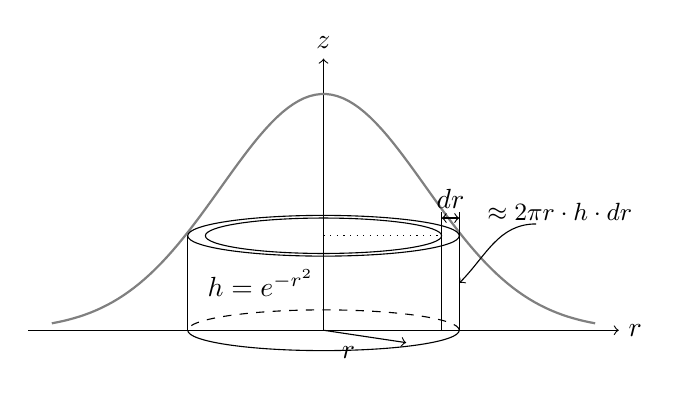
\begin{tikzpicture}[scale=1.5]
           
            \def\H{2.0}        
            \def\R{1.0}        
            \def\dR{0.15}      
            \def\ShellH{0.8}   
            \def\Y{0.15}      
    
            \draw[->] (-2.5, 0) -- (2.5, 0) node[right] {$r$};
            \draw[->] (0, 0) -- (0, \H+0.3) node[above] {$z$};
    
            \draw[gray, thick] plot[domain=-2.3:2.3, samples=100] (\x, {\H*exp(-\x*\x/1.5)});
            
            \draw[black, dashed] (\R+\dR, 0) arc (0:180:{\R+\dR} and {(\R+\dR)*\Y});

            \draw[black] (\R+\dR, 0) arc (0:-180:{\R+\dR} and {(\R+\dR)*\Y});
    
            \draw[black] (0, \ShellH) ellipse ({\R} and {\R*\Y});
            \draw[black] (0, \ShellH) ellipse ({\R+\dR} and {(\R+\dR)*\Y});
    
            \draw[black] (-\R-\dR, 0) -- (-\R-\dR, \ShellH);
            \draw[black] (\R, 0) -- (\R, \ShellH);
            \draw[black] (\R+\dR, 0) -- (\R+\dR, \ShellH);
    
            \draw[black, ->] (0, 0) -- (0.7*\R, -0.7*\R*\Y) node[midway, below left] {$r$};
            
            \draw[black] (\R, \ShellH) -- (\R, \ShellH+0.2);
            \draw[black] (\R+\dR, \ShellH) -- (\R+\dR, \ShellH+0.2);
            \draw[black, <->] (\R, \ShellH+0.15) -- (\R+\dR, \ShellH+0.15) node[midway, above] {$dr$};
            
            \draw[black, dashed] (0, 0) -- (0, \ShellH);
            \draw[black, dotted] (0, \ShellH) -- (\R, \ShellH);
            \node at (0, \ShellH/2) [left] {$h = e^{-r^2}$};
    
            \node at (2.0, 1.0) [align=left] {\small  $\approx 2\pi r \cdot h \cdot dr$};
            \draw[->, thin] (1.8, 0.9) to[out=180, in=45] (\R+\dR, \ShellH/2);
    
        \end{tikzpicture}
        \caption{高斯积分}
    \end{figure}

    于是
    \begin{align*}
        \int_{-\infty}^{+\infty}\int_{-\infty}^{+\infty}{\e}^{-(x^{2}+y^{2})}\d x\d y &= \int_{0}^{+\infty}{\e}^{-r^{2}} \cdot 2\pi r \d r \\
        &= \pi\int_{0}^{+\infty}{\e}^{-r^{2}}\d r^{2} \\
        &= \pi(-{\e}^{-r^{2}})\Big|_{0}^{+\infty} \\
        &= \pi
    \end{align*}
    从而原积分等于 $\sqrt{\pi}$。
\end{proof}

下面我们来计算 $V(d)$。方法是通过两种方式来计算积分：
\[
    \int_{-\infty}^{+\infty}\int_{-\infty}^{+\infty}\dots\int_{-\infty}^{+\infty}\e^{-(x_{1}^{2}+\dots+x_{d}^{2})}\d x_{1}\dots \d x_{d}
\]

一方面，利用之前的结果，上面的积分正是
\[
	\left(\int_{-\infty}^{+\infty}\e^{-x^{2}}\d x\right)^{d}=\pi^{\frac{d}{2}}
\]

另一方面，仍从几何上来看。令 $r^{2}=x_{1}^{2}+\dots+x_{d}^{2}$，整个体积依然是底面半径为 $r$ 的圆柱面的累加，只不过这里圆柱面的底面圆从 $2$ 维变成了 $d$ 维的。
\begin{align*}
	&\int_{-\infty}^{+\infty}\dots\int_{-\infty}^{+\infty}\e^{-(x_{1}^{2}+\dots+x_{d}^{2})}\d x_{1}\dots \d x_{d} \\
	= &\int_{0}^{+\infty}\e^{-r^{2}}\cdot A(d,r) \d r \\
    = &A(d) \int_{0}^{+\infty}\e^{-r^{2}}r^{d-1}\d r
\end{align*}

形如 $\displaystyle \int_0^{+\infty} x^n \e^{-x} \d x$ 的积分比较特别：
\begin{align*}
	\int_0^{+\infty} x^n \e^{-x} \d x &= \int_0^{+\infty} x^n \d(-\e^{-x}) \\
	&= -x^n \e^{-x} \bigg|_0^{+\infty} + \int_0^{+\infty} \e^{-x} \d x^n \\
	&= n \int_0^{+\infty} x^{n-1} \e^{-x} \d x
\end{align*}

令 $\Gamma(t+1) = \displaystyle \int_0^{+\infty} x^t \e^{-x} \d x$，则 $\Gamma(t+1) = t\Gamma(t)$，因而它是阶乘的推广。回到上面，由于
\begin{align*}
    \int_{0}^{+\infty}\e^{-r^{2}}r^{d-1}\d r &= \int_{0}^{+\infty}\e^{-r^{2}}(r^{2})^{\frac{d-1}{2}}\d r \\
    &= \int_{0}^{+\infty}\e^{-t} t^{\frac{d-1}{2}} \frac{1}{2} t^{-\frac{1}{2}} \d t \\
    &= \frac{1}{2}\int_{0}^{+\infty}\e^{-t}t^{\frac{d}{2}-1}\d t \\
	&= \frac{1}{2}\Gamma\left(\frac{d}{2}\right)
\end{align*}

所以
\[
    \pi^{\frac{d}{2}}=A(d)\cdot\frac{1}{2}\Gamma\left(\frac{d}{2}\right)
\]

由此得到结论：

\begin{theorem}
$d$ 维单位球的表面积和体积公式：
\[
	A(d)=\frac{2\pi^{\frac{d}{2}}}{\Gamma(\frac{d}{2})}
\]
\[
	V(d)=\frac{\pi^{\frac{d}{2}}}{\frac{d}{2}\Gamma(\frac{d}{2})}
\]
\end{theorem}

\section{高维单位球的更多性质}

\subsection{体积趋于0}

\begin{theorem}
    $d$ 维单位球的体积最终趋于 $0$，
    \[\lim_{d \to \infty} V(d) = 0\]
\end{theorem}

\begin{proof}
    使用 Stirling 公式，略。
\end{proof}

\subsection{体积集中在表面}

\begin{theorem}
    设 $S$ 为单位球，$(1-\epsilon)S=\{(1-\epsilon)x|x\in S\}$。
则至少有 $1-\e^{-\epsilon d}$ 比例的体积分布在 $S \setminus (1-\epsilon)S$ （“球壳”）中。
\end{theorem}

\begin{proof}
    \[
	   \frac{V((1-\epsilon)S)}{V(S)}=(1-\epsilon)^{d}\le \e^{-\epsilon d}
    \]
\end{proof}

\subsection{体积集中在“赤道”}

\begin{theorem}
    对 $c\ge1, d\ge3$，至少有 $1-\frac{2}{c}\e^{-\frac{c^{2}}{2}}$ 比例的体积满足 $|x^{(1)}|\le\frac{c}{\sqrt{d-1}}$。
\end{theorem}

\begin{proof}
    记 $S$ 为单位球。待定 $h \in (0, 1)$，令
    \[
	   H=\{x\in S \mid x^{(1)}\ge 0\}
    \]
    \[
	   A=\{x\in S \mid x^{(1)}\ge h\}
    \]

    \begin{figure}[htbp]
        \centering
        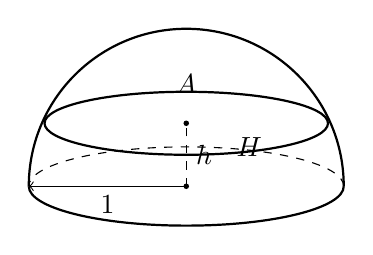
\begin{tikzpicture}[scale=1]
            \def\R{2} 
            \def\H{0.8}
            \def\r{1.8} 
            
            \draw[dashed] (\R,0) arc (0:180:{\R} and {0.5});
            \draw[thick] (\R,0) arc (0:-180:{\R} and {0.5});
            \draw[thick] (\R,0) arc (0:180:\R);
            \draw[thick] (0,\H) ellipse ({\r} and {0.4});
            
            \draw[dashed] (0,0) -- (0,\H) node[midway, right] {$h$};
            \fill (0,0) circle (1pt);
            \fill (0,\H) circle (1pt);

            \draw[->] (0,0) -- (-\R, 0) node[midway, below] {$1$};
            \node at (0, \H+0.5) {$A$};
            \node at (0.8, 0.5) {$H$};
        \end{tikzpicture}
        \caption{$H$ 与 $A$}
    \end{figure}
    
    先来放缩 $A$ 的体积：
    \begin{align*}
    	V(A) &= \int_{h}^{1}V(d-1,\sqrt{1-x^{2}})\d x \\
    	&= V(d-1)\int_{h}^{1}(1-x^{2})^{\frac{d-1}{2}}\d x \\
        &\le V(d-1)\int_{h}^{1}\e^{-\frac{d-1}{2}x^{2}}\d x \\
    	&\le V(d-1)\int_{h}^{+\infty}\frac{x}{h}\e^{-\frac{d-1}{2}x^{2}}\d x \\
    	&= \frac{V(d-1)}{h}\int_{h}^{+\infty}\e^{-\frac{d-1}{2}x^{2}}\d\left(\frac{x^{2}}{2}\right) \\
        &= \frac{V(d-1)}{h(d-1)}\e^{-\frac{d-1}{2}h^{2}}
    \end{align*}
    
    下面考虑 $H$ 的体积（$H$ 已经有了明确表达式为什么还要放缩？我们希望有一个包含 $V(d-1)$ 的界来和上面的消掉）。

    \begin{figure}[htbp]
        \centering
        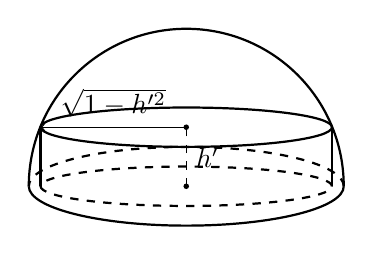
\begin{tikzpicture}[scale=1]
            \def\R{2}
            \def\H{0.75}
            \def\r{1.85}
            
            \draw[black, dashed, thick] (\R,0) arc (0:180:{\R} and {0.5});
            \draw[black, thick] (\R,0) arc (0:-180:{\R} and {0.5});
            \draw[black, thick] (\R,0) arc (0:180:\R);
            
            \draw[black, thick] (0,\H) ellipse ({\r} and {0.25});
            \draw[black, dashed, thick] (0,0) ellipse ({\r} and {0.25});
            \draw[black, thick] (-\r, 0) -- (-\r, \H);
            \draw[black, thick] (\r, 0) -- (\r, \H);
            
            \draw[black, dashed] (0,0) -- (0,\H) node[midway, right] {$h'$};
            \fill[black] (0,0) circle (1pt);
            \fill[black] (0,\H) circle (1pt);
            \draw[black, ->] (0,\H) -- (-\r, \H) node[midway, above] {$\sqrt{1-h'^2}$};
            
        \end{tikzpicture}
        \caption{$H$}
    \end{figure}
    
    如图所示， $V(H)$ 一定大于等于高为 $h'$ 的圆柱的体积（$h'$ 也待定），这样就有
    \begin{align*}
    	V(H) &\ge V(d-1,\sqrt{1-h'^{2}})\cdot h' = V(d-1)(1-h'^{2})^{\frac{d-1}{2}}h' \\
    	&\ge V(d-1)\left(1-\frac{d-1}{2}h'^{2}\right)h'
    \end{align*}
    令 $h=\frac{c}{\sqrt{d-1}}$, $h'=\frac{1}{\sqrt{d-1}}$，则有：
    \begin{align*}
    	V(A) &\le\frac{V(d-1)}{c\sqrt{d-1}}\e^{-\frac{c^{2}}{2}} \\
    	V(H) &\ge V(d-1)\cdot\left(1-\frac{1}{d-1}\cdot\frac{d-1}{2}\right)\cdot\frac{1}{\sqrt{d-1}}=\frac{V(d-1)}{2\sqrt{d-1}}
    \end{align*}
    综上可得：
    \[
    	\frac{V(A)}{V(H)}\le\frac{2}{c}\e^{-\frac{c^{2}}{2}}
    \]
\end{proof}

\subsection{球上的点几乎两两正交}

\begin{theorem}
    在单位球中随机取 $n$ 个点 $x_1, \dots, x_n$, 有 $1 - O(\frac{1}{n})$ 的概率使得
    \begin{enumerate}
    	\item $\|x_i\| \ge 1 - \frac{2 \ln n}{d} \quad \forall i$.
    	\item $|\langle x_i, x_j \rangle| \le \frac{\sqrt{6 \ln n}}{\sqrt{d-1}} \quad \forall i \neq j$.
    \end{enumerate}
\end{theorem}

\begin{proof}
    利用 Union Bound.
    \begin{align*}
    	\Pr\left[\exists i, \|x_i\| < 1-c\right] &\le n \Pr\left[\|x_1\| < 1-c\right] \\
    	&= n \cdot (1-c)^d < n \e^{-cd}
    \end{align*}
    只要使 $n \e^{-cd} \le \frac{1}{n}$ 即可, 取 $c = \frac{2 \ln n}{d}$.
    
    对于第二个不等式, 将 $x_1$ 旋转到 $(1, 0, \dots, 0)$ 所在的方向, 则 $|\langle x_1, x_j \rangle| \le |x_j^{(1)}|$. 利用刚刚的结果，
    \begin{align*}
    	\therefore \Pr\left[\exists i \neq j, |\langle x_i, x_j \rangle| > \frac{c}{\sqrt{d-1}}\right] 
    	&\le n^2 \Pr\left[|\langle x_1, x_2 \rangle| > \frac{c}{\sqrt{d-1}}\right] \\
    	&\le n^2 \Pr\left[|x_1^{(1)}| > \frac{c}{\sqrt{d-1}}\right] \\
    	&\le n^2 \cdot \frac{2}{c} \e^{-\frac{c^2}{2}} \\
    	&\le n^2 \e^{-\frac{c^2}{2}}
    \end{align*}
    只要让 $n^2 \e^{-\frac{c^2}{2}} \le \frac{1}{n}$, 即 $\e^{-\frac{c^2}{2}} \le \frac{1}{n^3}$.
    取 $c = \sqrt{6 \ln n}$ 即可.
\end{proof}

\subsection{体积集中在中心的立方体内}

\begin{theorem}
    单位球至少一半的体积集中在中心在原点的边长 $\frac{4\sqrt{\ln d}}{\sqrt{d-1}}$ 的正方体内部。
\end{theorem}

\begin{proof}
    \[
    	\Pr\left[\exists i, |x^{(i)}| > \frac{c}{\sqrt{d-1}}\right] \le d\cdot\frac{2}{c}\e^{-\frac{c^{2}}{2}}
    \]
    取 $c=2\sqrt{\ln d}$，则上界为 $d \cdot \frac{1}{\sqrt{\ln d}}\cdot\frac{1}{d^{2}} < \frac{1}{d} < \frac{1}{2}$。
\end{proof}

这也为 $V(d)\rightarrow 0$ 提供了另一种证明。

注：看上去与球的体积集中在表面矛盾？实际上这个立方体在 $d$ 较大的时候并不是完全位于球的内部的，会伸出来很多“刺”，类似于一个“海胆”，参见书上的这幅图：

\begin{figure}
    \centering
    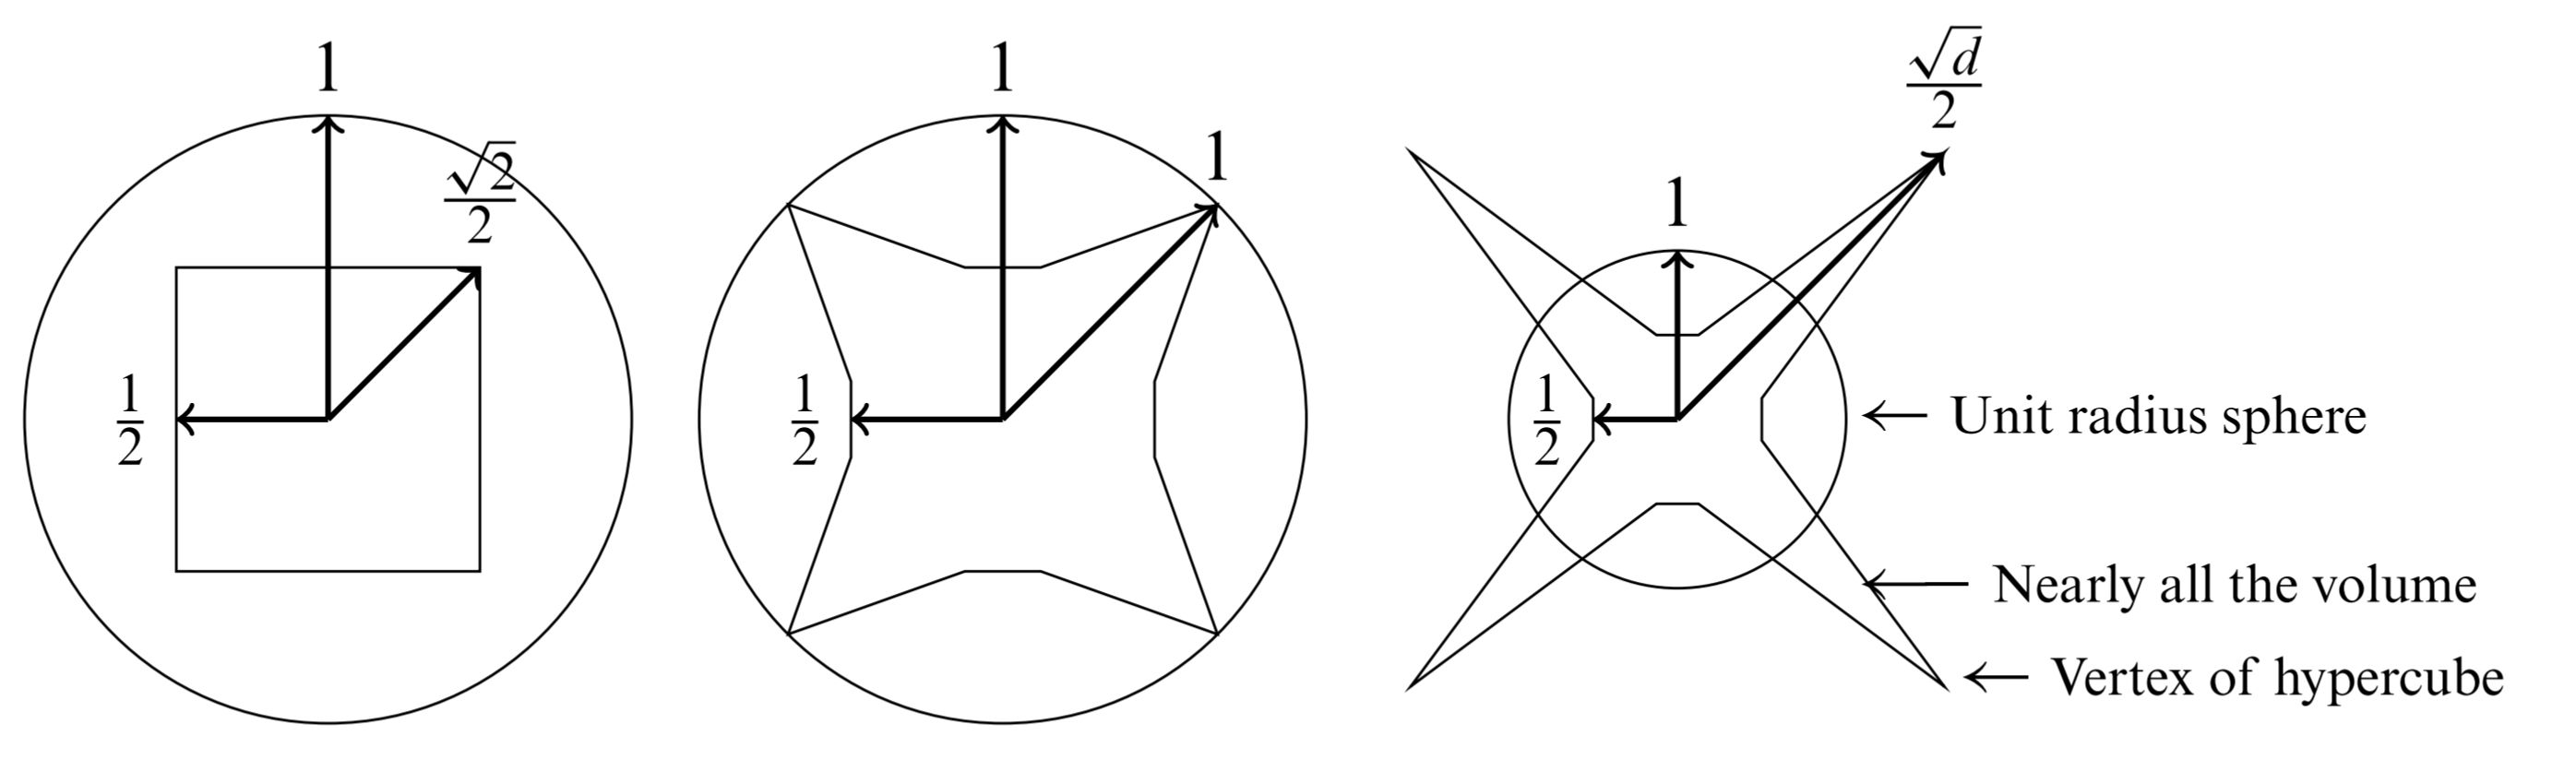
\includegraphics[width=1.0\linewidth]{imgs/sphere_and_cube.jpg}
    \caption{$2$, $4$, $d$ 维的球面与立方体的示意图}
\end{figure}

\section{随机投影，Johnson-Lindenstrauss 引理}

先简单引入一个工具：

\begin{theorem}
    对任意正整数 $d$，独立地从标准高斯中采样 $x=(x_{1},\dots,x_{d})$，则存在正常数 $c$，使得对 $\beta\le\sqrt{d}$，至少有 $1-3\e^{-c\beta^{2}}$ 的概率使
    \[
    	\|x\| \in [\sqrt{d}-\beta, \sqrt{d}+\beta].
    \]
\end{theorem}

这个定理称为“高斯圆环定理”，此处不证。其实很符合直觉：$\E[\|x\|^{2}]=\E[x_{1}^{2}+\dots+x_{d}^{2}]=d\E[x_{1}^{2}]=d$，故 $x$ 大概率分布在半径 $\sqrt{d}$ 附近的“圆环”中。

接下来我们关心这样一件事情，对于 $k \ll d$，给定 $\mathbb{R}^{d}$ 中的 $n$ 个点 $v_{1}, \dots, v_{n}$，能否找到一个投影 $f: \mathbb{R}^{d}\longrightarrow \mathbb{R}^{k}$ 使得在降维的同时尽量保持这 $n$ 个点间的距离？
也即对 $\epsilon\in(0,1)$，$\forall i,j$：
\[
	(1-\epsilon)\|v_{i}-v_{j}\| \le \|f(v_{i})-f(v_{j})\| \le (1+\epsilon)\|v_{i}-v_{j}\| ?
\]

为了解决这件事，我们需要使用所谓的\textbf{概率方法}：要证明存在满足性质 $P(x)$ 的对象 $x$，只要证明以某种方式随机取 $x$，$\Pr[P(x)]>0$ 即可。

如何来构造这种随机？我们利用标准高斯分布，随机选取 $u_{1},\dots,u_{k} \in \mathbb{R}^{d}$ i.i.d $\sim N(0,1)$。定义 $f: \mathbb{R}^{d}\longrightarrow\mathbb{R}^{k}$，
\[
	v \mapsto (\langle v,u_{1}\rangle, \dots, \langle v,u_{k}\rangle)
\]
我们可以证明，这样的 $f$ 大概率能把距离保持地很好：

\begin{theorem}
    对于 $0<\epsilon<1$，$\forall n \in \mathbb{N}^*$，$\exists c>0$，当 $k\ge\frac{3}{c\epsilon^{2}}\ln n$ 时，对 $\mathbb{R}^{d}$ 中任何 $n$ 个点，如上定义的 $f$ 有至少 $1-\frac{3}{2n}$ 的概率使得 $\forall i,j$
    \[
    	(1-\epsilon)\sqrt{k}\|v_{i}-v_{j}\| \le \|f(v_{i})-f(v_{j})\| \le (1+\epsilon)\sqrt{k}\|v_{i}-v_{j}\|
    \]
\end{theorem}

\begin{proof}
    $f$ 是线性映射，$f(v_{i})-f(v_{j})=f(v_{i}-v_{j})$。实际上只需要考虑对 $\mathbb{R}^{d}$ 中的 $n^{2}$ 个点，
    \[
    	\|f(v)\| \in [\|v\|(1-\epsilon), \|v\|(1+\epsilon)]
    \]
    对于 $f(v)$ 的分量 $\langle v, u_{i} \rangle = \sum v^{(j)}u_{i}^{(j)}$，
    由于 $u$ 的每个坐标分量均独立地服从高斯分布，故 $\langle v, u_{i} \rangle$ 也服从高斯分布，并且可以计算出
    \begin{align*}
    	\E[\langle v, u_{i} \rangle] &= 0 \\
    	\Var[\langle v, u_{i} \rangle] &= \sum (v^{(j)})^{2}=\|v\|^{2}
    \end{align*}
    即 $\langle v, u_{i} \rangle \sim N(0,\|v\|^{2})$。
    
    令 $v \leftarrow \frac{v}{\|v\|}$，不妨设 $\|v\|=1$。此时我们已经知道 $\|f(v)\| \approx \sqrt{k}$。在高斯圆环定理中取$\beta=\sqrt{k}\epsilon$，则 $\exists c>0$，至少有 $1-3\e^{-ck\epsilon^{2}}$ 的概率使
    \[
    	\|f(v)\| \in [\sqrt{k}(1-\epsilon), \sqrt{k}(1+\epsilon)]
    \]
    
    利用 Union Bound，只需
    \[
    	\frac{n^2}{2} \cdot 3\e^{-ck\epsilon^{2}} < \frac{3}{2n}
    \]
    $k > \frac{3}{c\epsilon^{2}}\ln n$ 已足够。
\end{proof}

修改 $f: v \mapsto \frac{1}{\sqrt{k}}(\dots)$，这样的 $f$ 就符合了我们最开始的动机。